\titledquestion{Question \thequestion: Network MP Question} % Simon

For all parts of this question, consider the following network topology.\\
Assume that the default firewall policy allows all traffic.
\begin{center}
    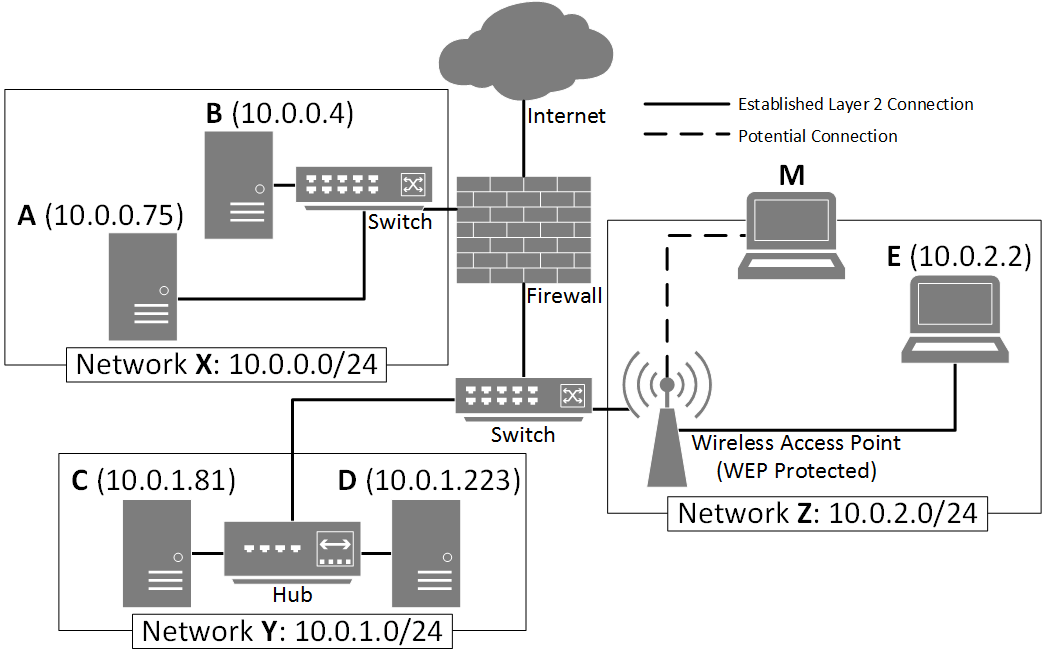
\includegraphics[scale = 0.55]{topology} \\
\end{center}

\begin{parts}

\part[1]
Assume that there is an active unencrypted TCP session between Hosts A and C and that every host on the network knows the IP address of A and C.
\\
Which other host(s) on the network can eavesdrop on this communication by performing passive sniffing only?

\begin{solutionorbox}[0.5in]
D\\
+1 correct
\end{solutionorbox}

\part[2]
Assume that there is an active unecrypted TCP session between Hosts B and C and that every host on the network knows the IP address of B and C.\\
\\
What technique can Host A use to eavesdrop on this communication? Name the technique and briefly describe it.

\begin{solutionorbox}[1in]
MAC flooding, filling up switch's memory with random MAC addresses; ARP spoofing, changing victim's ARP table\\
+1 correct name\\
+1 correct explanation
\end{solutionorbox}

\pagebreak

\part[4]
Assume that there is an active unencrypted TCP session between Hosts B and E and that Host M is not part of any network or associated with the wireless access point.

\begin{subparts}
\subpart
How should Host M's wireless adapter be configured to eavesdrop on this communication?
\begin{solutionorbox}[0.5in]
monitor mode\\
+1 correct
\end{solutionorbox}

\subpart
Host M detects other wireless network activities nearby.\\
\\
What two pieces of wireless network information can be provided to airodump-ng so that only the packets from Network Z are captured?
\begin{solutionorbox}[0.5in]
BSSID (or MAC address of AP), channel number\\
+1 each correct name
\end{solutionorbox}

\subpart
When inspecting the captured packets with Wireshark, the user of Host M is unable to see the contents because they are encrypted by WEP.\\
\\
Which wireless network information does the user need to see the plaintext version of the payload?
\begin{solutionorbox}[0.5in]
WEP key\\
+1 correct
\end{solutionorbox}

\end{subparts}

\pagebreak

\part[4]
Consider the following packet trace from the network:\\

{
\centering
\begin{tabular}{|l|l|l|l|l|l|}
\hline
\textbf{src\_ip}  & \textbf{src\_port}  & \textbf{dst\_ip}  & \textbf{dst\_port}  & \textbf{tcp\_flags} \\ \hline
\multicolumn{5}{|c|}{...} \\ \hline
10.0.0.4          & 21                  & 10.0.1.223        & 50678               & {[}SYN, ACK{]}      \\ \hline
10.0.1.223        & 50678               & 10.0.0.4          & 21                  & {[}ACK{]}           \\ \hline
10.0.0.4          & 21                  & 10.0.1.223        & 50678               & {[}PSH, ACK{]}      \\ \hline
\multicolumn{5}{|c|}{...} \\ \hline
10.0.0.4          & 20                  & 10.0.1.223        & 43583               & {[}SYN{]}           \\ \hline
10.0.1.223        & 43583               & 10.0.0.4          & 20                  & {[}SYN, ACK{]}      \\ \hline
10.0.0.4          & 20                  & 10.0.1.223        & 43583               & {[}ACK{]}           \\ \hline
\multicolumn{5}{|c|}{...} \\ \hline
10.0.0.4          & 20                  & 10.0.1.223        & 43583               & {[}FIN, ACK{]}      \\ \hline
10.0.1.223        & 43583               & 10.0.0.4          & 20                  & {[}FIN, ACK{]}      \\ \hline
10.0.0.4          & 20                  & 10.0.1.223        & 43583               & {[}ACK{]}           \\ \hline
\multicolumn{5}{|c|}{...} \\ \hline
10.0.1.223        & 50678               & 10.0.0.4          & 21                  & {[}FIN, ACK{]}      \\ \hline
10.0.0.4          & 21                  & 10.0.1.223        & 50678               & {[}FIN, ACK{]}      \\ \hline
10.0.1.223        & 50678               & 10.0.0.4          & 21                  & {[}ACK{]}           \\ \hline
\multicolumn{5}{|c|}{...} \\ \hline
\end{tabular}\\
}

\vspace{.2in}

Assuming that this is a trace of FTP file transfer, answer the following questions:
\begin{subparts}
\subpart
What is the IP address of the FTP server?

\begin{solutionorbox}[0.5in]
10.0.0.4\\
+1 correct
\end{solutionorbox}

\subpart
What port number did the server use to transfer data (i.e. FTP-DATA port)?

\begin{solutionorbox}[0.5in]
20\\
+1 correct
\end{solutionorbox}

\subpart
Is this FTP transfer done in active or passive mode? Give one reason why you came to this conclusion.
\begin{solutionorbox}[1in]
active mode, because FTP-DATA is port 20 or data transfer is initiated by the server.\\
+1 correct answer\\
+1 correct explanation
\end{solutionorbox}

\end{subparts}

\pagebreak

\part[3]
Based on the diagram at the beginning of Question 4, create inbound firewall rules that satisfy the following conditions:
\begin{itemize}
\item Deny all inbound traffic to Network X by default.
\item Allow inbound traffic to Network X for HTTP.
\item Allow Network Y to SSH to Network X.
\end{itemize}

\vspace{.05in}

Fill in the table following the directions below:
\begin{itemize}
\item You may or may not need to use all rows.
\item Assume that rules are processed from the top down.
\item For \textbf{Source} and \textbf{Destination} columns, you may write either the network name or its IP address range in CIDR notation to specify a range of IP addresses or a network.
\item For \textbf{Application} column, you may write either the service name or its port number.
\end{itemize}

{
\centering
\begin{tabular}{|p{4cm}|p{4cm}|p{3cm}|p{3cm}|}
\hline
\textbf{Source} & \textbf{Destination}  & \textbf{Application}  & \textbf{Action} \\      \hline
                &                       &                       &                 \\[2ex] \hline
                &                       &                       &                 \\[2ex] \hline
                &                       &                       &                 \\[2ex] \hline
                &                       &                       &                 \\[2ex] \hline
\end{tabular}\\

}
\vspace{.1in}

Example (does not apply to our topology):\\

{
\centering
\begin{tabular}{|p{4cm}|p{4cm}|l|p{2cm}|p{1cm}|}
\hline
\textbf{Source}             & \textbf{Destination}  & \textbf{Application}  & \textbf{Action} \\ \hline
Network W (or 10.0.7.0/24)  & 10.0.4.4              & SMTP (or 25)          & Allow           \\ \hline
\end{tabular}\\
}

\vspace{.1in}

\begin{solution}[3in]

+1 for each correct row\\
-0.5 if Deny all is not the first row\\
-1 for each of other incorrect rows\\

{
\centering
\begin{tabular}{|l|l|l|l|l|}
\hline
\textbf{Source}   & \textbf{Destination}  & \textbf{App}    & \textbf{Action} \\ \hline
Any               & X or 10.0.0.0/24      & Any             & Deny            \\ \hline
Any               & A or 10.0.0.75        & HTTP or 80      & Allow           \\ \hline
Y or 10.0.1.0/24  & A or 10.0.0.75        & SSH or 22       & Allow           \\ \hline
\end{tabular}\\
}

\end{solution}

\end{parts}
